\documentclass[12pt,a4paper,twoside]{article}
\input{185.dat}
\usepackage{gensymb}
\usepackage{amsthm}
\usepackage{float}
\usepackage{siunitx}
\usepackage{amssymb}
\usepackage{float}
\usepackage{enumerate}
\usepackage{listings}
\usepackage{mathtools}
\usepackage[none]{hyphenat}
\usepackage{physics}
\newcommand\ddfrac[2]{\frac{\displaystyle #1}{\displaystyle #2}}
%\renewcommand{\familydefault}{\sfdefault}
\usepackage{booktabs,tabularx}
\usepackage{tabulary}
\renewcommand{\tabularxcolumn}{m}
\usepackage{listings}
\PassOptionsToPackage{hyphens}{url}\usepackage{hyperref}
\usepackage{color, colortbl}
\definecolor{cyan}{rgb}{0.85,0.89,0.95}
\renewcommand{\familydefault}{\sfdefault}

\begin{document}

\begin{titlepage}
\begin{center}
\vspace*{\fill}

\Huge{ Live-Feed-over-LAN Pressure Sensor (LoLAN-PresS) Documentation} \\

\qquad
\qquad

\normalsize{Members: \\ 
Kenneth V. Domingo \\
Rhei Joven G. Juan \\
Rene L. Principe Jr. \\ \medskip
App Physics 185 }

\vspace*{\fill}
\end{center}
\end{titlepage}

\setcounter{page}{1}

\section{Overview}\label{sec:overview}
\medskip
The Live-Feed-over-LAN Pressure Sensor (LoLAN-PresS) is an implementation of velostat pressure/bend sensor which runs on an ESP8266-based microcontroller. On the hardware end, the sensor broadcasts through a local area network (LAN) using a pre-set IP address. On the software end, the feed can be retrieved, processed, and displayed in real-time through any Python interpreter on a device connected on the same network. The program depends on the following Python libraries:

\begin{itemize}

\item Numpy
\item Matplotlib
\item Scipy
\item URLlib

\end{itemize}

\section{Hardware setup}\label{sec:hardware}\medskip
The hardware of LoLAN-PresS requires the following items along with their costs during Q2 2019:

\begin{table}[h!]
	\centering
	\caption{Cost of required materials.}
	\begin{tabulary}{\linewidth}{CCCRR}
	Qty & Item & Source & Cost/pc (PhP) & Subtotal (PhP) \\ \hline
	1 & Velostat sheet & circuit.rocks & 349.00 & 349.00 \\
	1 & NodeMCU 1.0 Lua WiFi Board & circuit.rocks & 325.00 & 325.00 \\
	1 & PCB - H503B & DEECO & 40.00 & 40.00 \\
	& & & \textbf{TOTAL} & 714.00
	\end{tabulary}
\end{table}

The velostat may come in small patches or a large sheet. Cutting this into the desired shape results in little change in its properties. The following hardware setup instructions are for the microcontroller specified in the materials, but can easily be adjusted for any WiFi microcontroller of choice:

\begin{enumerate}
    \item Cut the velostat sheet either in small circular patches or a heel-shaped patch.
    \item Tape a copper wire one one side of the sheet such that it roughly follows the shape of the sheet. Connect this to the \texttt{A0}/analog pin of the microcontroller.
    \item Do the same for the other side of the sheet, but make sure the wires do not touch. Connect this to the \texttt{GND}/ground pin of the microcontroller.
    \item Tape a third wire on any side of the sheet (it no longer needs to follow the shape of the sheet). Make sure it also does not touch any other wire. Connect this to the \texttt{3V3} (3.3 V) pin of the microcontroller.
\end{enumerate}

\begin{figure}[h!]
	\centering
	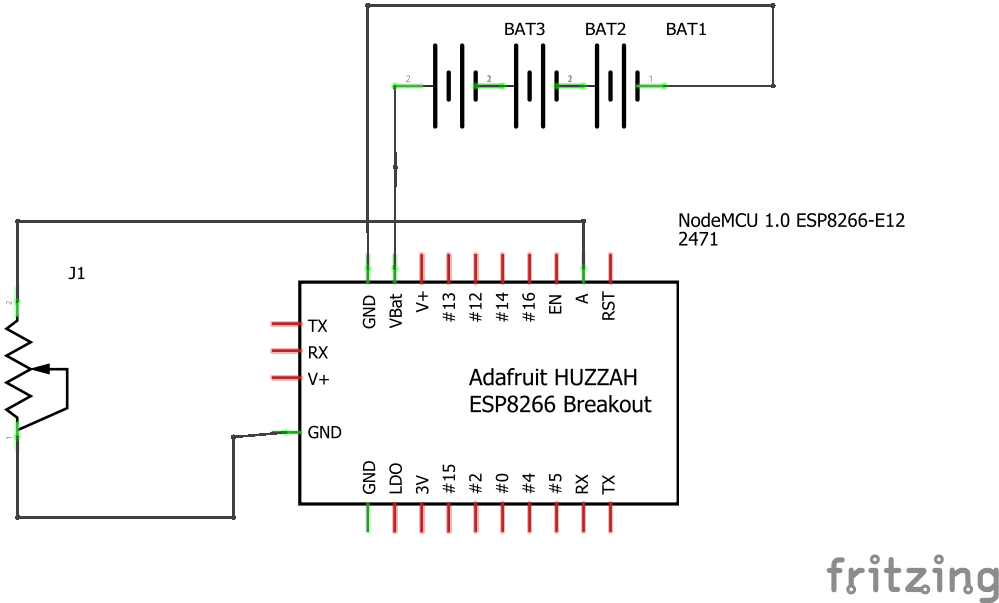
\includegraphics[width=0.75\linewidth]{setup.png}
	\caption{Schematic of the hardware setup. The element labelled \texttt{J1} is the velostat sheet. The elements labelled \texttt{BAT1}-\texttt{BAT3} can be any DC source, as long as it can deliver sufficient current and the output voltage does not exceed 5V.}
	\label{fig:schematic}
\end{figure}

\section{Software setup}\label{sec:software}\medskip
The following is a documentation of the program and how to set it up.

\subsection{The \texttt{PressureSensor} class}
The \texttt{PressureSensor} class contains the functions and attributes needed for communication with the microcontroller and live display of the analog data.

\subsubsection{\texttt{\footnotesize{PressureSensor}\normalsize{.\_\_init\_\_(url, calibration)}}}
Instantiates the \texttt{Spectrometer} object and takes the calibration arguments.

\begin{table}[H]
    \caption{Program initialization.}
    \begin{tabular}{>{\columncolor{cyan}}p{2in} p{4in}}
        \hline
        \textbf{Parameters} & \texttt{url : str} \\
        &   Local IP address of the microcontroller. \\ 
        & \texttt{calibration : str} \\
        &   Filename of the data to be used for calibration of voltage-to-force. \\ \hline
    \end{tabular}
    \label{tab:prog-init}
\end{table}

\subsubsection{\texttt{\footnotesize{PressureSensor}\normalsize{.plot\_calibration()}}}
Displays the calibration curve and the voltage-to-force equation.

\subsubsection{\texttt{\footnotesize{PressureSensor}\normalsize{.runlive()}}}
Starts the live feed and saves all currently received data every 3 seconds to \texttt{datalog.npy}.

\subsection{\texttt{characterization(filename, width, polyorder, lim)}}
The \texttt{characterization} function allows the retrieval and processing of saved \texttt{.npy} files for processing later on.

\begin{table}[H]
    \caption{Program initialization.}
    \begin{tabular}{>{\columncolor{cyan}}p{2in} p{4in}}
        \hline
        \textbf{Parameters} & \texttt{filename : str} \\
        &   Filename of the data to be processed. Accepts \texttt{.txt}, \texttt{.log}, and \texttt{.npy} formats. \\ 
        & \texttt{width : int} \\
        &   Specifies the filter window length of the Savitzky-Golay filter. \\ 
        & \texttt{polyorder : int} \\
        &	Specifies the order of the polynomial used to fit the samples in the Savitzky-Golay filter. \\
        & \texttt{lim : tuple} \\
        &	Specifies the index range of the data to be processed. \\ \hline
    \end{tabular}
    \label{tab:prog-characterize}
\end{table}

The full code is available in the Appendix. The following software setup instructions are for the microcontroller specified in the materials, but can easily be adjusted for any WiFi microcontroller of choice:

\begin{enumerate}
    \item Connect the microcontroller to a laptop/computer using a micro-USB connector.
    \item Go to the GitHub project repository (see Appendix) and clone the LoLAN-PresS repository onto a local drive.
    \item Open \texttt{IP\_test/IP\_test.ino} in Arduino IDE. Go to line 102 (line beginning with \texttt{start()}).
    \item Replace the first string with the name of the local network's SSID. Replace the second string with the network password (leave it blank if there is no password). Do not remove the quotation marks.
    \item Upload the program to the microcontroller. Once complete, disconnect the microcontroller from the computer.
    \item Connect a powerbank to the micro-USB socket of the microcontroller and wait a few seconds for it to initialize.
    \item On a computer, open the interface of your network router (the address is usually \texttt{192.168.0.1}, else the local address is usually printed on the router itself. If all else fails, contact your network administrator). Search the network for the IP address of the microcontroller. It should begin with \texttt{ESP}, followed by a few numbers.
    \item Open \texttt{IP\_test.ipynb} in Jupyter Notebook and initialize cells 1--3. Go to line 1 of cell 4 and replace the variable \texttt{url} with the IP address of the microcontroller.
    \item Run cell 4. If everything has been set up correctly, the live feed should begin. If it does not, check if all instructions starting with step 1 have been followed correctly. Also ensure all the dependencies have been installed.
    \item Data from the live feed is saved every 3 seconds to \texttt{datalog.npy}. To perform post-live feed analysis, simply open the datalog using the function \texttt{characterization()} and input the desired parameters.
\end{enumerate}

\section{Demonstration}

\begin{figure}[h!]
	\centering
	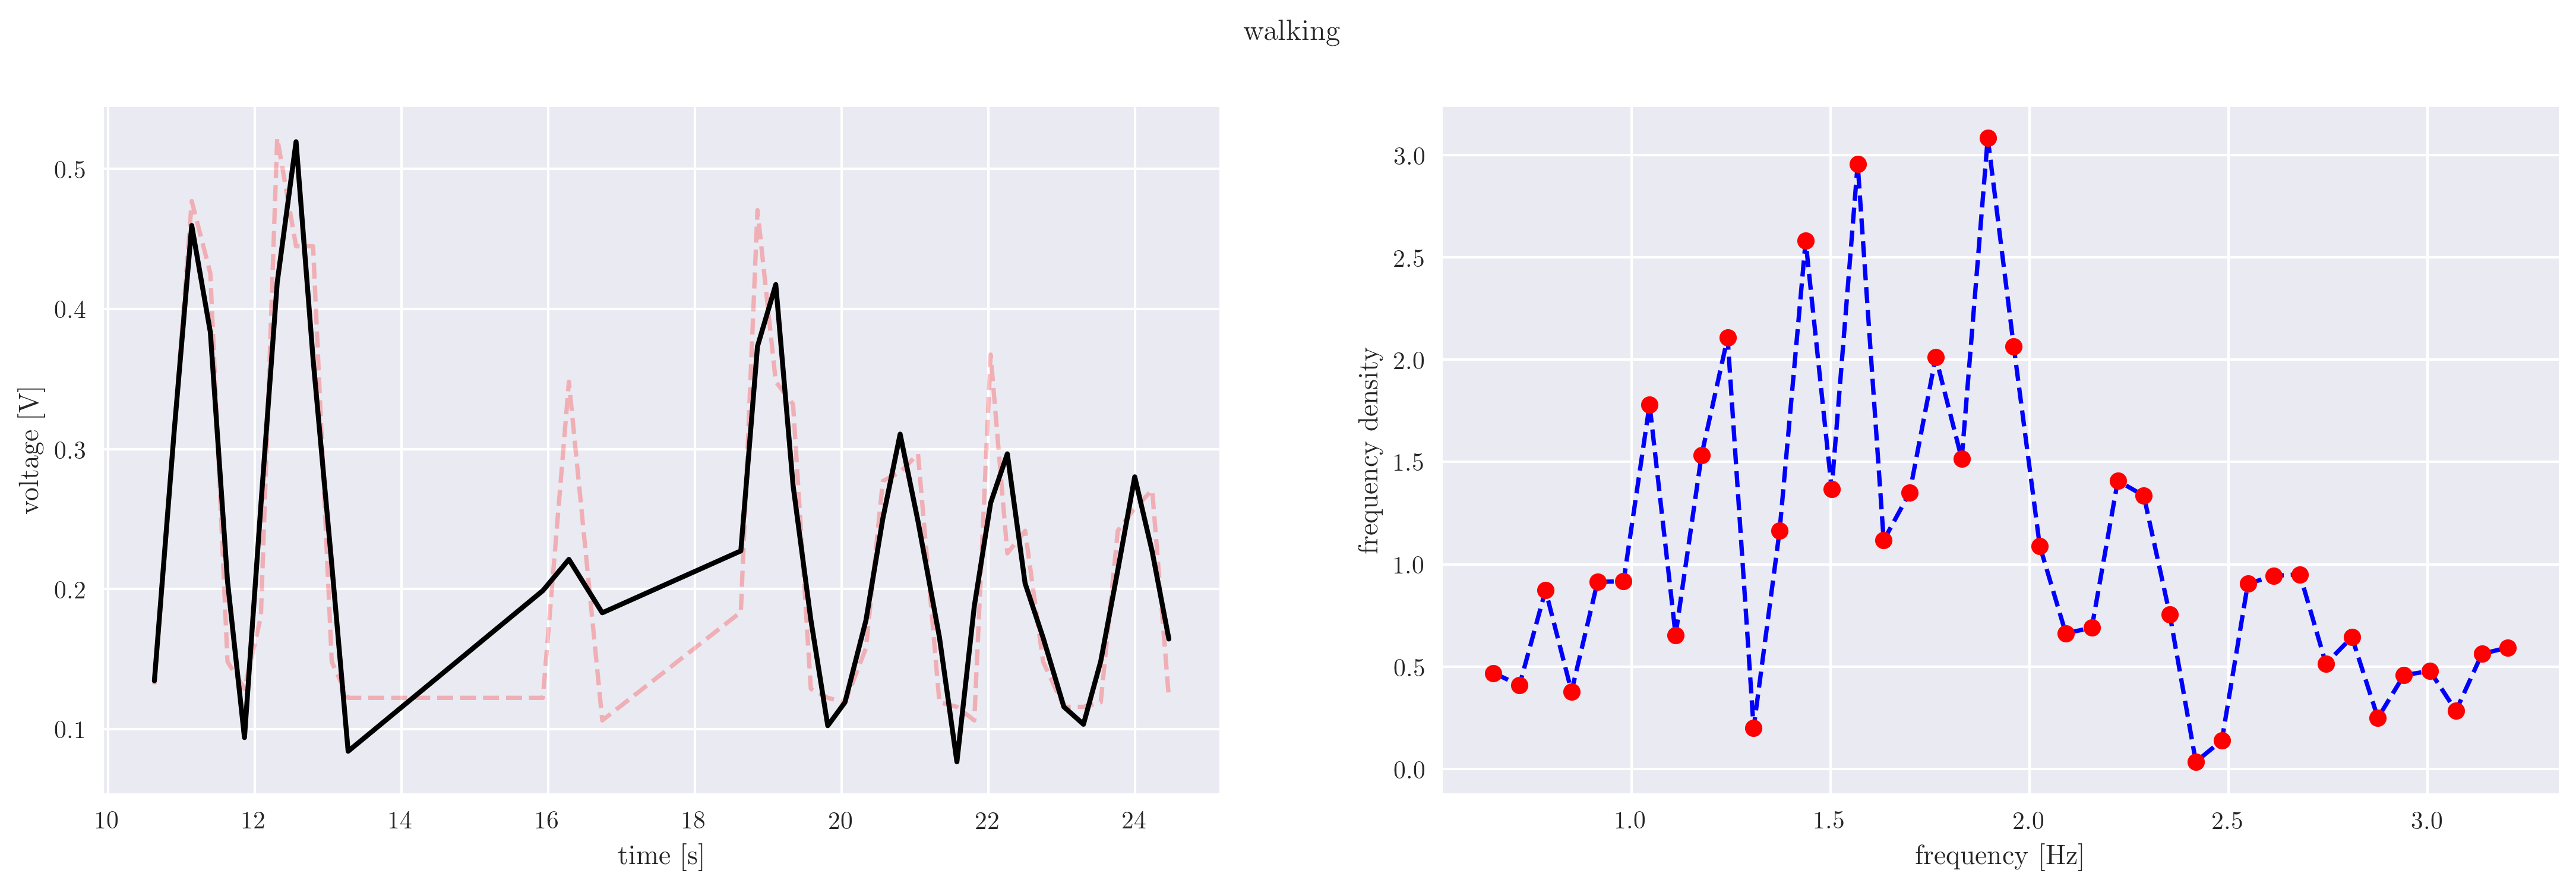
\includegraphics[width=\linewidth]{walking.png}
	\caption{Walking.}
	\label{fig:walking}
\end{figure}

\begin{figure}[h!]
	\centering
	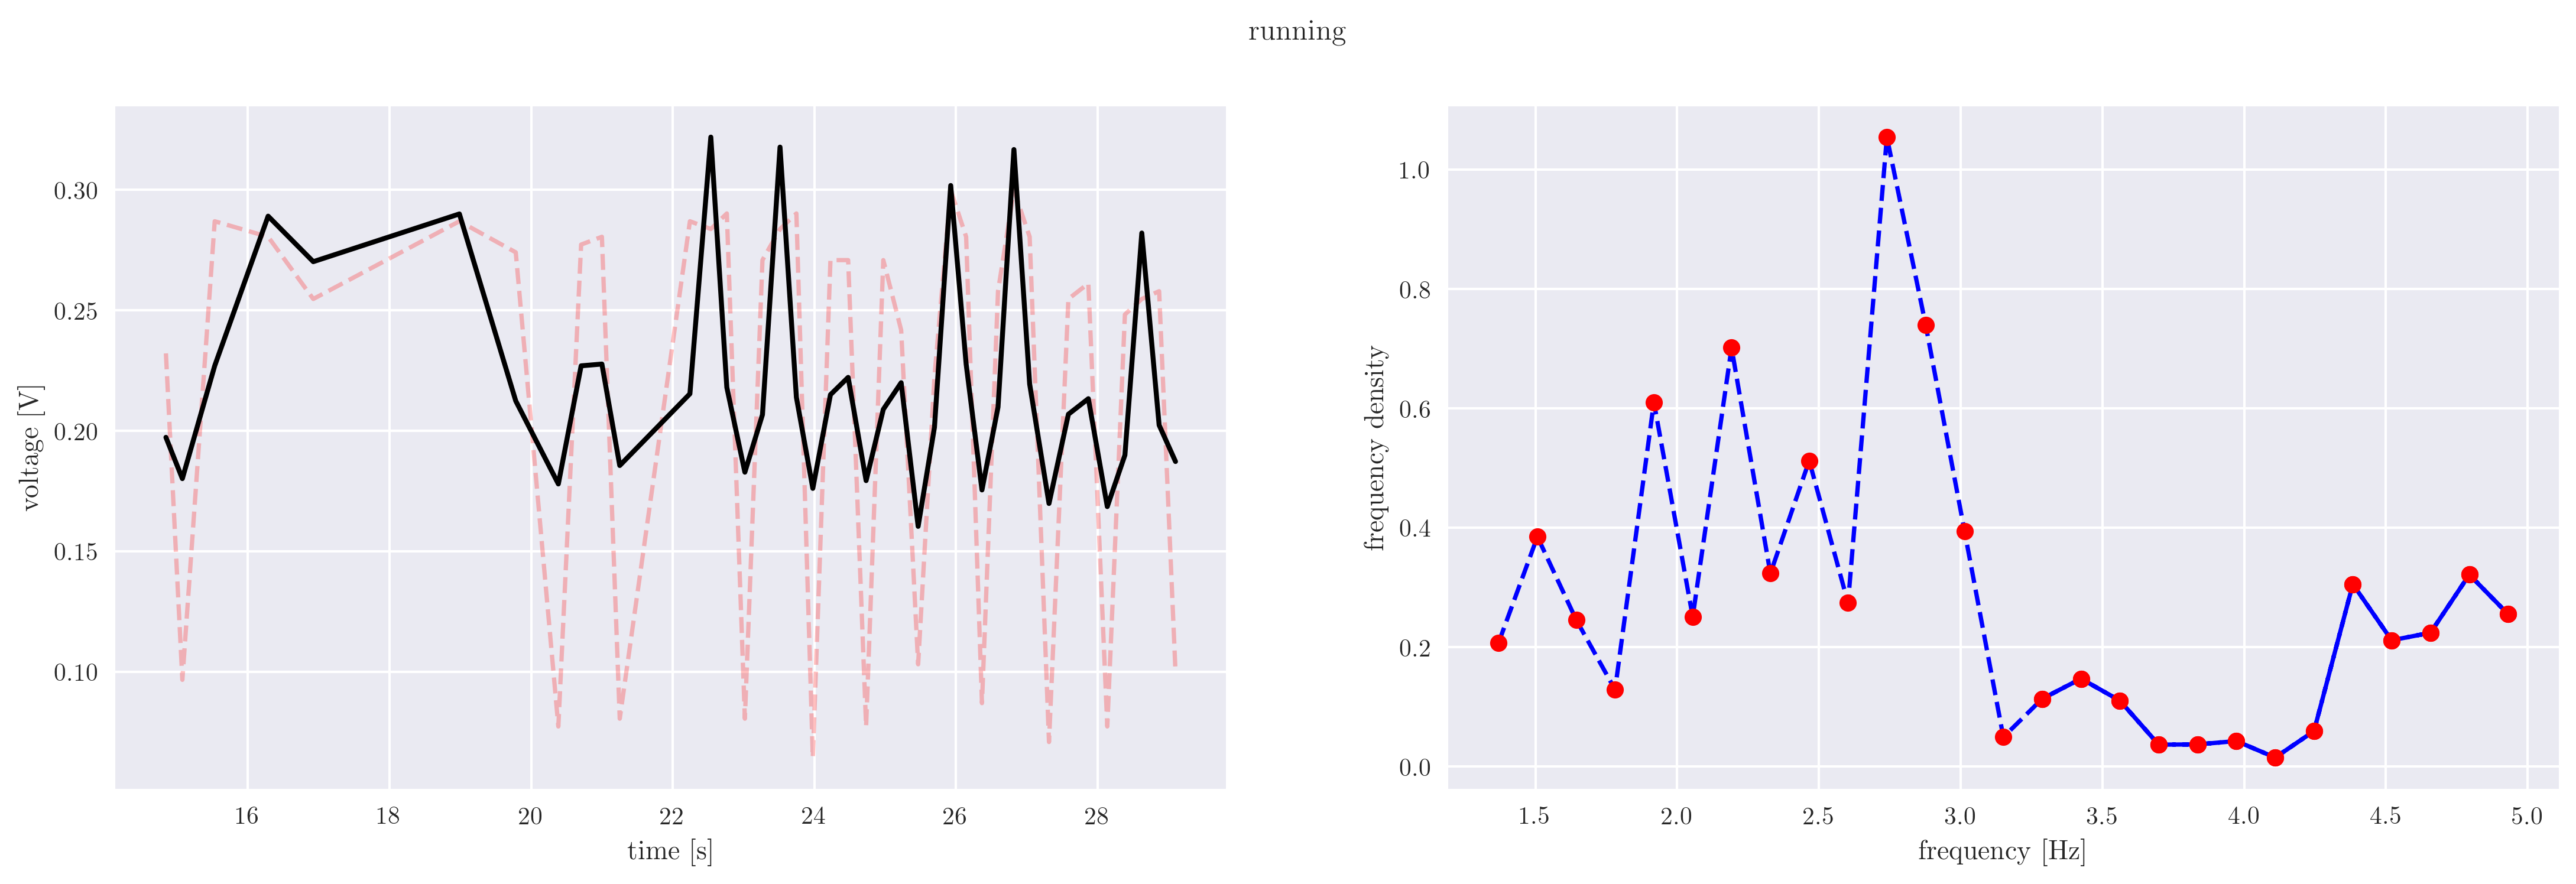
\includegraphics[width=\linewidth]{running.png}
	\caption{Running.}
	\label{fig:Running}
\end{figure}

\begin{figure}[h!]
	\centering
	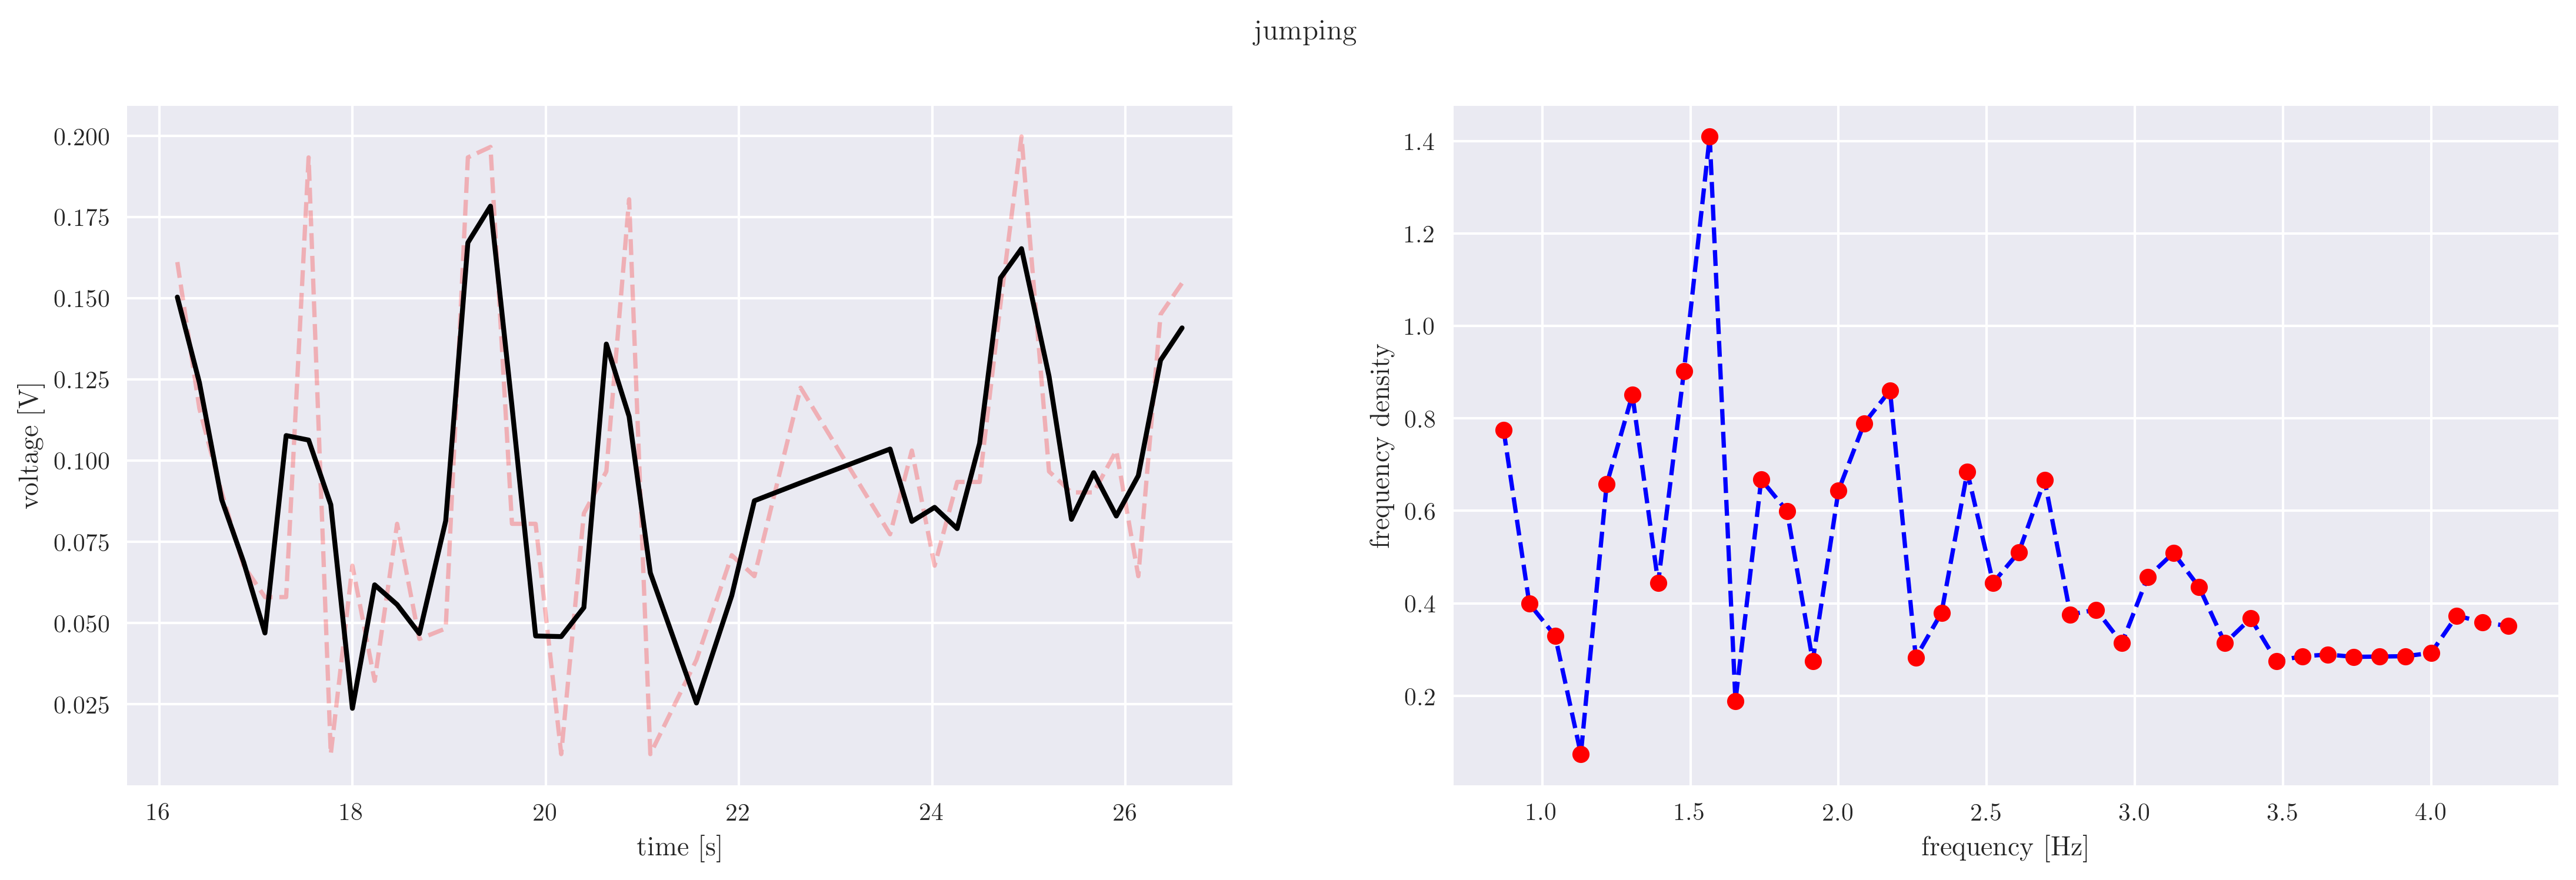
\includegraphics[width=\linewidth]{jumping.png}
	\caption{Jumping.}
	\label{fig:jumping}
\end{figure}

\clearpage

\section*{Appendix}
Source code: \\
\url{https://colab.research.google.com/drive/1MEt__i0g5831f0d1dX7pcIu3H4YR8fnU} \\

\noindent
GitHub repository: \\
\url{https://github.com/kvdomingo/LoLAN-PresS}

%\bibliographystyle{spp-bst}
%\bibliography{bibfile}

%\raggedbottom

%\pagebreak
%\pagebreak[3]
\iffalse
\newpage

\renewcommand\thefigure{A\arabic{figure}} 
\setcounter{figure}{0}
\fi %removing this will break the code for some reason

\end{document}

